\section{Gantt chart}
We identify the tasks of our project and their schedule, using the Gantt chart below.
		\begin{center}
			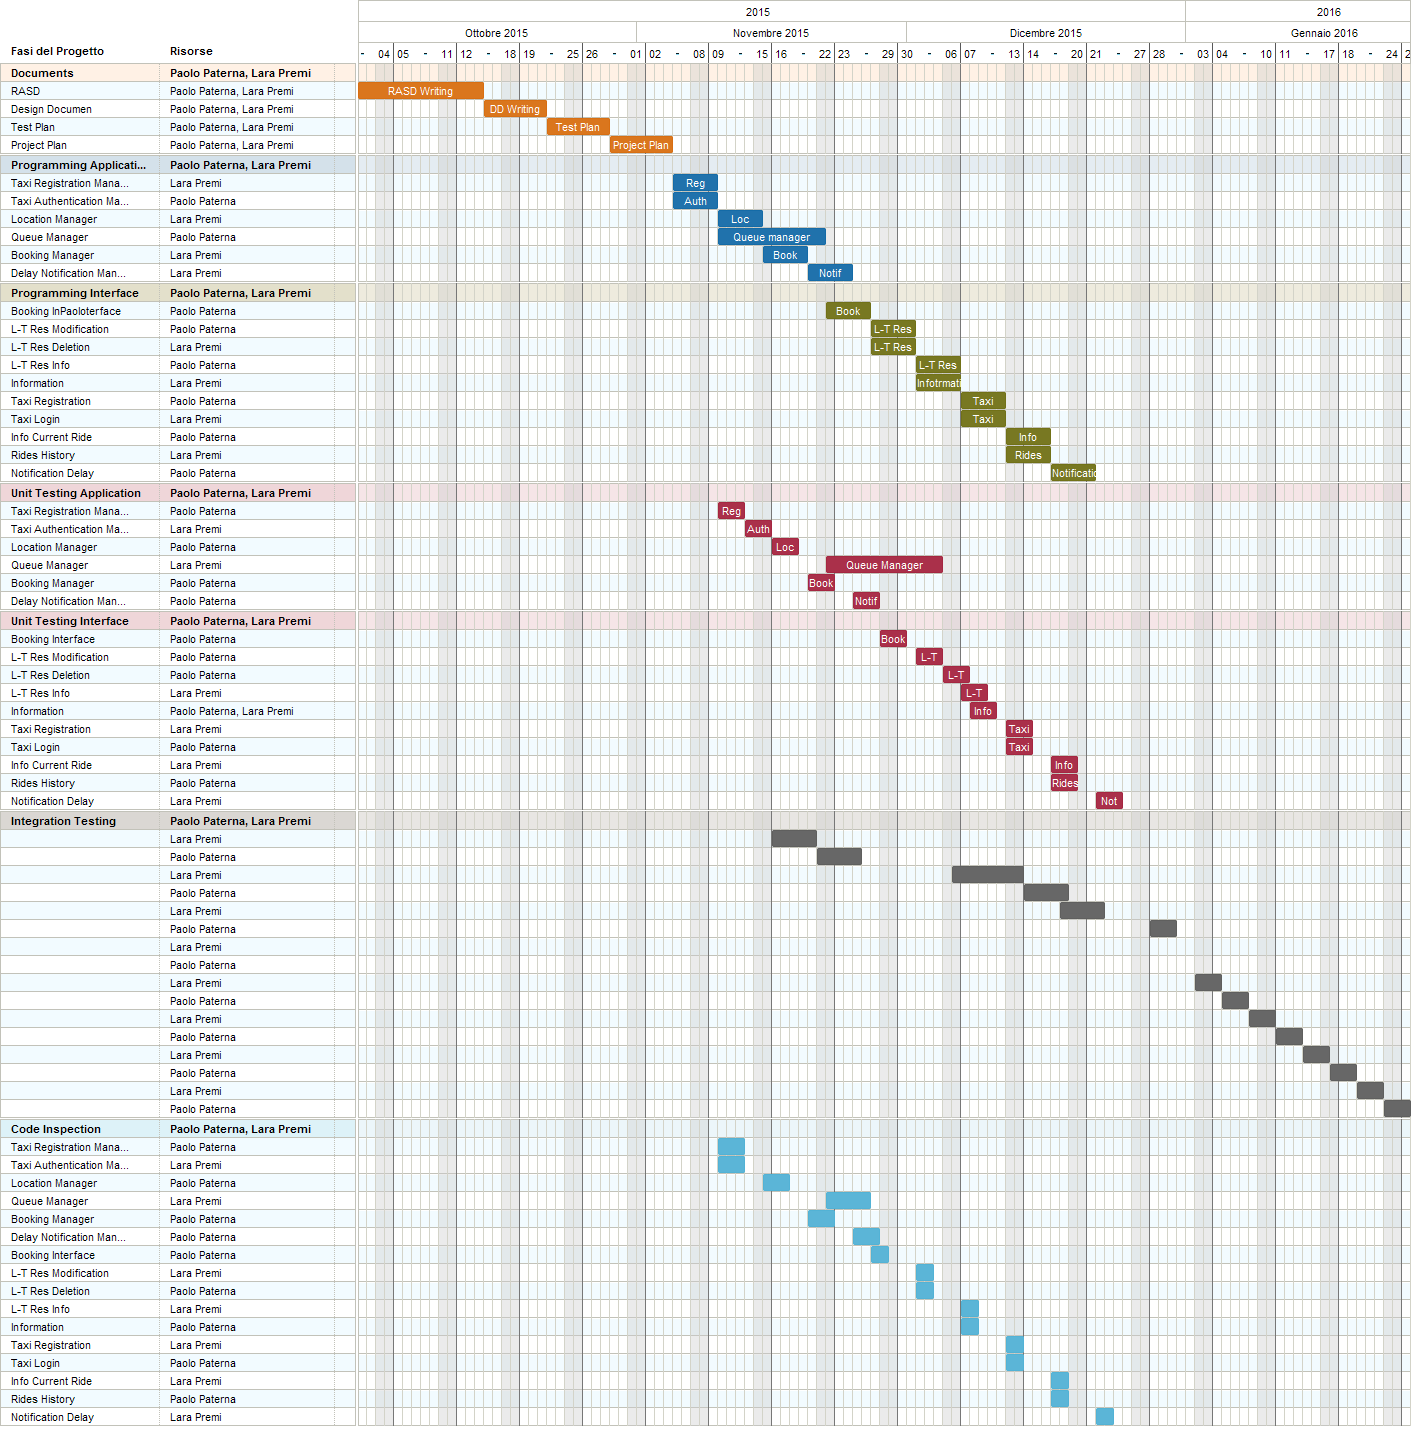
\includegraphics[width=1\textwidth]{./images/myTaxiService.png}
		\end{center}
		
\newpage
\section{Risks}
We have considered two risks. First of all, it could happen that the project staff is ill at critical time, during the work: this risk is characterized by a moderate probability to occur and it can have serious effects. To solve it, the team will be reorganize, impling that there will be more overlap of work and people therefore will understand each other's jobs.
The second risk on which we have focused on is that the database used in the system cannot process as many transactions per second as expected: this risk is characterized by a moderate probability to happen and it can have serious effects, like the first risk that we have said before. In this case, the staff will investigate the possibility of buying a higher-performance database.
	